%% This is file `elsarticle-template-1-num.tex',
%%
%% Copyright 2009 Elsevier Ltd
%%
%% This file is part of the 'Elsarticle Bundle'.
%% ---------------------------------------------
% \documentclass[preprint,12pt]{elsarticle}
%% Use the option review to obtain double line spacing
%% \documentclass[preprint,review,12pt]{elsarticle}

%% Use the options 1p,twocolumn; 3p; 3p,twocolumn; 5p; or 5p,twocolumn
%% for a journal layout:
% \documentclass[final,1p,times]{elsarticle}
% \documentclass[final,1p,times,twocolumn]{elsarticle}
\documentclass[final,3p,times]{elsarticle}
%% \documentclass[final,3p,times,twocolumn]{elsarticle}
%% \documentclass[final,5p,times]{elsarticle}
% \documentclass[final,5p,times,twocolumn]{elsarticle}

%% The graphicx package provides the includegraphics command.
% \usepackage{graphicx}
%% The amssymb package provides various useful mathematical symbols
% \usepackage{amssymb}
%% The amsthm package provides extended theorem environments
%% \usepackage{amsthm}

%% The lineno packages adds line numbers. Start line numbering with
%% \begin{linenumbers}, end it with \end{linenumbers}. Or switch it on
%% for the whole article with \linenumbers after \end{frontmatter}.
% \usepackage{lineno}

%% \biboptions{comma,round}

% \biboptions{}
\usepackage{nameref}
\usepackage{siunitx}


% include graphics
\usepackage{graphicx}
\graphicspath{ {figures/} }

% include pdfs
\usepackage{pdfpages}


%% using bibtex with biber
\usepackage[
    backend=biber,
    style=nature,
    sortlocale=de_DE,
    url=false,
    doi=true,
    eprint=false
]{biblatex}
\addbibresource{reference.bib}


\journal{}
\begin{document}


\begin{frontmatter}

%% Title
\title{Investigating semi-automated ki67 scoring efficacy}
%% Authors
\author[molgen]{Peiqi Wang}
\author[music]{Tian Yu Liu}
\author[cf]{Susan J. Done\corref{cor}}
\ead{Susan.Done@uhn.ca}
%% address
\cortext[cor]{Principal corresponding author}
\address[molgen]{Department of Molecular Genetics and Microbiology, University of Toronto, Canada}
\address[music]{Faculty of Music, Univeristy of Toronto, ON, Canada}
\address[cf]{The Campbell Family Institute for Breast Cancer Research, Canada}

\begin{abstract}
300words, work done, result obtained, conclusions drawn. filled in later


% \begin{itemize}
% \item Bullet point one
% \item Bullet point two
% \end{itemize}
%
% \begin{enumerate}
% \item Numbered list item one
% \item Numbered list item two
% \end{enumerate}

% \begin{table}[h]
% \centering
% \begin{tabular}{l l l}
% \hline
% \textbf{Treatments} & \textbf{Response 1} & \textbf{Response 2}\\
% \hline
% Treatment 1 & 0.0003262 & 0.562 \\
% Treatment 2 & 0.0015681 & 0.910 \\
% Treatment 3 & 0.0009271 & 0.296 \\
% \hline
% \end{tabular}
% \caption{Table caption}
% \end{table}


\end{abstract}

\begin{keyword}
ki67 \sep breast cancer
\end{keyword}

\end{frontmatter}

%%
%% Start line numbering here if you want
%%
\linenumbers

%% main text
\section*{Introduction}

Ki-67 is a human nuclear protein detected exclusively in the active phases of the cell cycle, namely $G_1$, $S$, $G_2$, and mitosis, while absent in the resting $G_0$ phase.\cite{Gerdes1984} It is expressed in virtually cells of every tissue origin and is highly sensitive to cell cycle changes, making it an ideal marker for quantifying uncontrolled proliferation, a hallmark of cancer. Unsurprisingly, Ki-67 immunohistochemical (IHC) staining of human neoplasmic cell has emerged as a rapid and cost-effective analytics capable of determining the growth fraction of tumour cell populations,  \cite{Scholzen2000} The use of Ki-67 labelling index, or the percentage of Ki-67-positive cells, has great prognostic potential particularly in carcinomas of the breast, where a multitude of studies report the use of Ki-67 labeling index in predicting disease free/overall survival and tumour recurrence \cite{Stuart-Harris2005, DeAzambuja2007, Petrelli2015} as well as in guiding neoadjuvant chemotherapy. \cite{Jones2009, Nishimura2010, Fasching2011} Practically, Ki-67 labeling index may contribute to improved tumour grading, where proliferation is routinely assessed using mitotic count. \cite{VanDiest2004} Additionally, it may serve as a feasible and cost-effective alternative to gene signature based assessments such as OncotypeDx in cancer subtyping when used in conjunction with established breast histopathological markers. \cite{Cuzick2011}

Despite its apparent value in cancer prognosis, widespread use of Ki-67 labeling index in clinical pathology is hampered by the lack of standardization and suffers from substantial intra- and interobserver variability. \cite{Dowsett2011a, Polley2013a} Although recommendations and quidelines exist in an effort to harmonize such variability, \cite{Polley2015} the choice of scoring methods and selection of cut-off for Ki-67 positivity remain a subject of debate. One promising approach to the problem utilizes digital image analysis (DIA), which ensures automaticity, repeatability and reproducibility. However, aforementioned characteristics do not guarantee objectivity; Differences in image segmentation and algorithm used could still give rise to variability. \cite{Tadrous2010} Some DIA methods were reported to agree comparably with \cite{Mohammed2012} or even outperform visual assessments; \cite{Laurinavicius2014, Stalhammar2016} Others suggested that DIA methods were less reliable and prognostic. \cite{Chabot-Richards2011} It is apparent that inter-algorithmic variability is high and performance is context dependent. Therefore, there is a great need in evaluating the validity and reliability of existent DIA methods so as to identify major sources of variability and potential solutions.

In this study, we evaluated two digital image analysis methods - Aperio ePathology and Definiens Tissue Studio. The former is a semi-automated pipeline requiring explicitly image segmentation; while the latter automates the process by calibrating against a few test cases. We assessed reliability of the two DIA methods by reporting their agreement to a set of manual scores previously identified to be a predictor of ipsilateral breast relapse in the the Toronto-British Columbia (TBC) trial patient cohort. \cite{Liu2015}  Additionally, we measured inter-rater reliability for the Aperio system. We also explored ways in which errors were introduced to the system and how best to mitigate them.

\section*{Materials and Methods}

\subsection*{Sample Collection}
A subset of patient cohort from the TBC trial were used for this study. \cite{Liu2015} The TBC trial consists of node-negative patients who were older than 50 years of age randomly assigned to receive tamoxifen alone or tamoxifen and breast radiotherapy after breast-conserving surgery. \cite{Fyles2009} Tissue microarrays were constructed using a triplicate of \SI{0.6}{\milli\metre} tumour cores from formalin-fixed, paraffin-embedded blocks. A total of 6 TMA blocks, amounting to 278 cases, where used for subsequent IHC and image analysis. TMA blocks were cut in \SI{0.5}{\micro\metre} sections, stained with 1:500 dilution SP6 (NeoMarker) and counter-stained with hematoxylin.

\subsection*{Scoring Methodologies}

\subsubsection*{Manual Assessment}
A trained individual, assigned as rater 1, counted the number of brown staining for at least 100 cells within tumour hot spot, or areas in which Ki-67 most frequently expressed, for each core. The total number of nucleus and positively stained nucleus over the span of three cores were summed and the Ki-67 labeling index was calculated for each case. 10\% of the samples were randomly chosen and rescored for quality assurance. As the scores resulting from this set of manual assessment was clinically significant in predicting ipsilateral breast relapse, they were used as a reference value to be compared with other scoring methods.

\subsubsection*{Digital Image Analysis (DIA)}
To assess intra-algorithmic variability of the DIA methods, specifically the Aperio system, 2 trained individuals, assigned as rater 1 and rater 2, independently marked tumour region of interest (ROI) for proper image segmentation. Settings, such as minimum nucleus radius and staining intensity threshold, for the algorithm were subjectively adjusted for by another experienced pathologist and used in both set of images. Segmented images were analyzed to quantify inter-rater reliability when using a DIA method. To assess the agreement of DIA method to the manual score reference, the same set of images were analyzed using the Definiens system in addition to the Aperio system. In this case, a technician, assigned as rater 3, segmented images in a few cases, which calibrated the software to perform automatic segmentation. Minor adjustments were made to correct for faulty segmentation.

\subsection*{Statistics}
Data distribution for different scoring methods were visualized using boxplot, accompanied by summary statistics. Bland-Altman plot was used to visualize agreements between scores from the two DIA methods in relation to manual score reference. \cite{Bland1986} 95\% confidence interval for the limits of agreement as well as the mean difference was calculated based on an alpha of 0.05. Two methods were considered unbiased and precise if the mean difference centered about zero with a small standard deviation. \cite{Hanneman2008} To correct for positive skewness, Ki-67 labeling indices were log base 2 transformed after incrementing by 1\% for subsequent statistical calculation. Inter-rater reliability (IRR) was quantified using a two-way mixed, average-measures intraclass correlation coefficient (ICC) to assess the degree that raters provide absolute agreement in their ratings of Ki-67 labeling index using the Aperio system. \cite{Shrout1979} An ICC close to 1 represents high reliability. Similarly, ICC was used to assess the degree that results from the two DIA methods agree with that of the manual score reference. Conger generalized Kappa were calculated based on a set of commonly used cut-offs for Ki-67 labeling index to evaluate the practicality of consistent classification using manual assessment as reference. \cite{Conger1980}


\section*{Results}

\subsubsection*{Overall Distribution}
Boxplot of untransformed Ki-67 labeling index as well as summary statistics presented in Figure~\ref{boxplot}, and Table~\ref{boxStat}. The Aperio system tended to overestimate Ki-67 labeling index; whereas the Definiens system showed a similar distribution to manual score reference.

\subsubsection*{Agreement of DIA methods to Manual Score Reference}

Bland-Altman plot for every DIA method compared to manual score reference was presented in Figure~\ref{baplot}. Relevant statistics to the plots were tabulated in Table~\ref{baStat}. It was apparent that the Aperio system systematically overestimated Ki-67 labeling index by a large margin in both scoring instances. The Definiens system faired better in introducing minimal bias, but still exhibited non-negligible variability. The discrepancy in agreements of the two DIA methods could be largely attributable to subjective setting assignments in addition to varying algorithm implementation. When there was no reliable benchmark to fallback on, unbiased image segmentation could be challenging and may require multiple calibration cycles to reduce measurement errors.

ICC of two raters using the Aperio system when compared directly to the manual score reference was 0.173 (95\%CI -0.245 $\sim$ 0.459) and 0.439 (95\%CI -0.258 $\sim$  0.72) respectively, representing poor to moderate agreements. ICC of rater using the Definiens system when compared to the manual score reference was 0.892 (95\%CI 0.841 $\sim$ 0.924). High degree of agreement was achieved, suggesting that the Ki-67 labeling index was scored similarly using manual assessment and a DIA method. Unsurprisingly, ICC for the two DIA methods differ, a direct consequence of the systematic bias previously shown in the Bland-Altman plot.

It may be misleading to solely measure absolute agreement, as ultimately cases would be classified into clinically relevant groups based on the Ki-67 labeling index. Kappa statistics calculated using cut-offs from a meta-analysis study were listed in Table~\ref{kappaStat}. \cite{Petrelli2015} With a 14\% cut-off used to distinguish  luminal B from luminal A tumours, \cite{Cheang2009} the kappa value obtained using the Definiens system was 0.65, suggesting a substantial agreement in making clinically relevant classifications. \cite{Landis1977} With a hypothetical 25\% cut-off used to distinguish {'}luminal B-like{'} tumours proposed in the recent St. Gallen Breast Cancer Conference, \cite{Coates2015} the two DIA methods achieved fair to moderate agreement with kappa value of 0.35, 0.57 respectively.


\subsubsection*{Inter-rater Reliability Using a DIA Method}
ICC between two raters using the the Aperio system was 0.538 (95\%CI: 0.31-0.68) The resulting ICC could be considered moderate, suggesting that a substantial amount of error was introduced in the process of image segmentation in addition to heterogeneous tumour biology. \cite{Cicchetti1994} Additionally, Kappa statistics for two raters using the Aperio system indicated slight to fair agreement as presented in Table~\ref{kappaStat}. \cite{Landis1977}


\section*{Discussions}
interpretation of significance of findings, relate to other works, further research directions


The experiment is still comparing to manual scores, which is still indirect and subject to an additional layer of error. so future direction could be evaluate and compare clinical features with old and new methods.


\printbibliography


\newpage
%% figures and tables
\begin{figure}
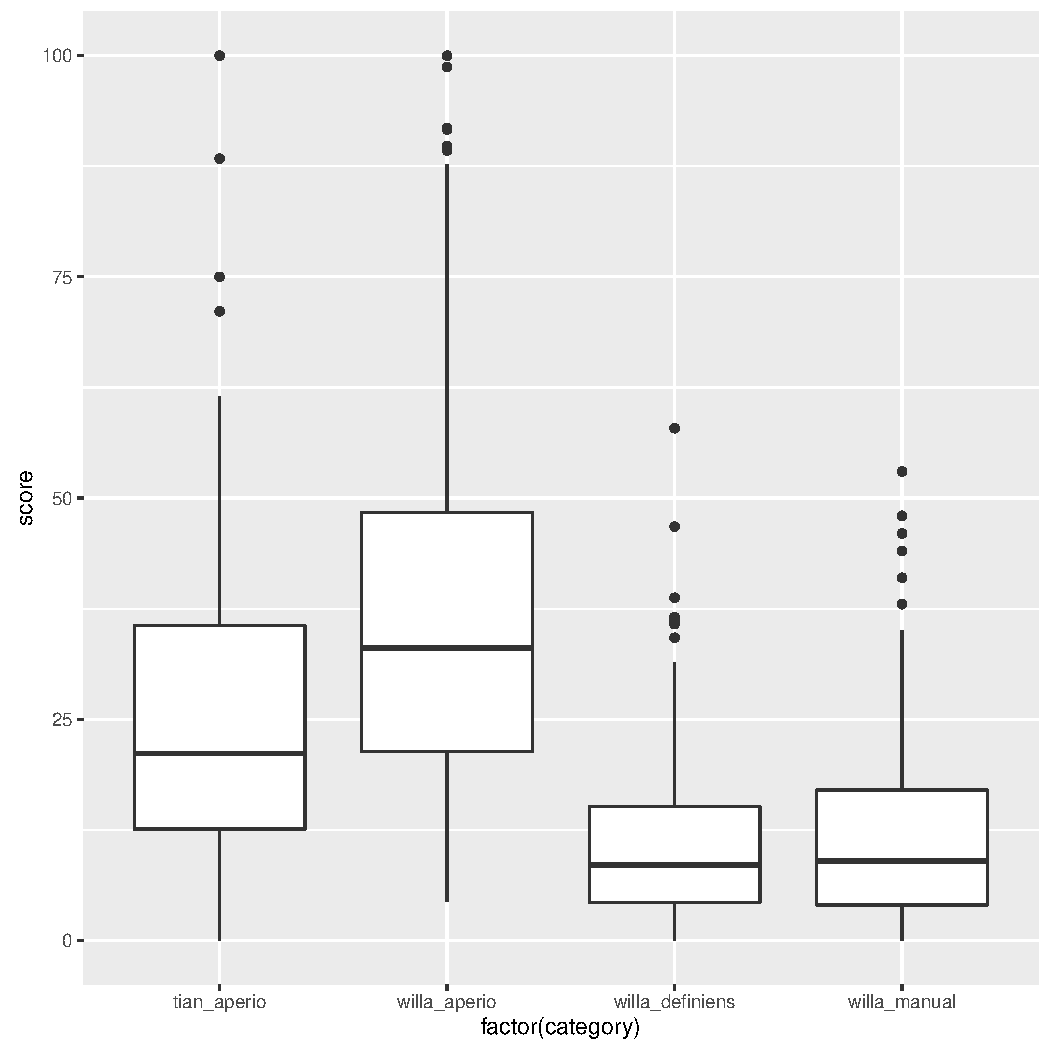
\includegraphics[width = 11cm]{boxplot}
\centering
\caption{{\bf Summary boxplot of Ki-67 labeling index}}
\label{boxplot}
\end{figure}

\begin{figure}
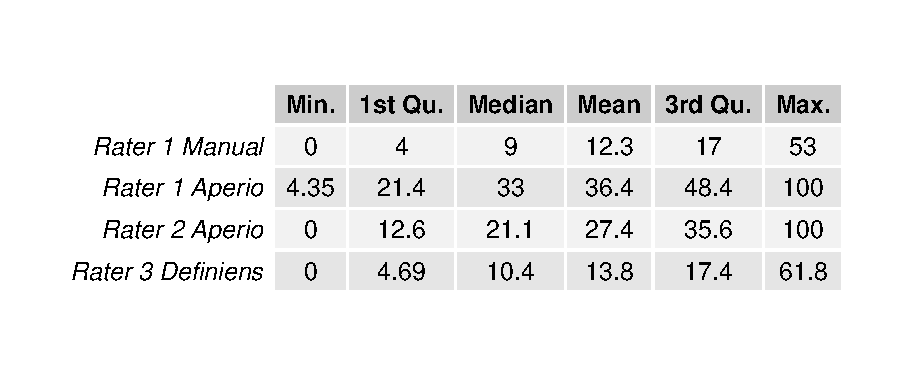
\includegraphics[width = 11cm]{boxStat}
\centering
\caption{{\bf Summary statistics for log2-transformed Ki-67 labeling index}}
\label{boxStat}
\end{figure}


\begin{figure}
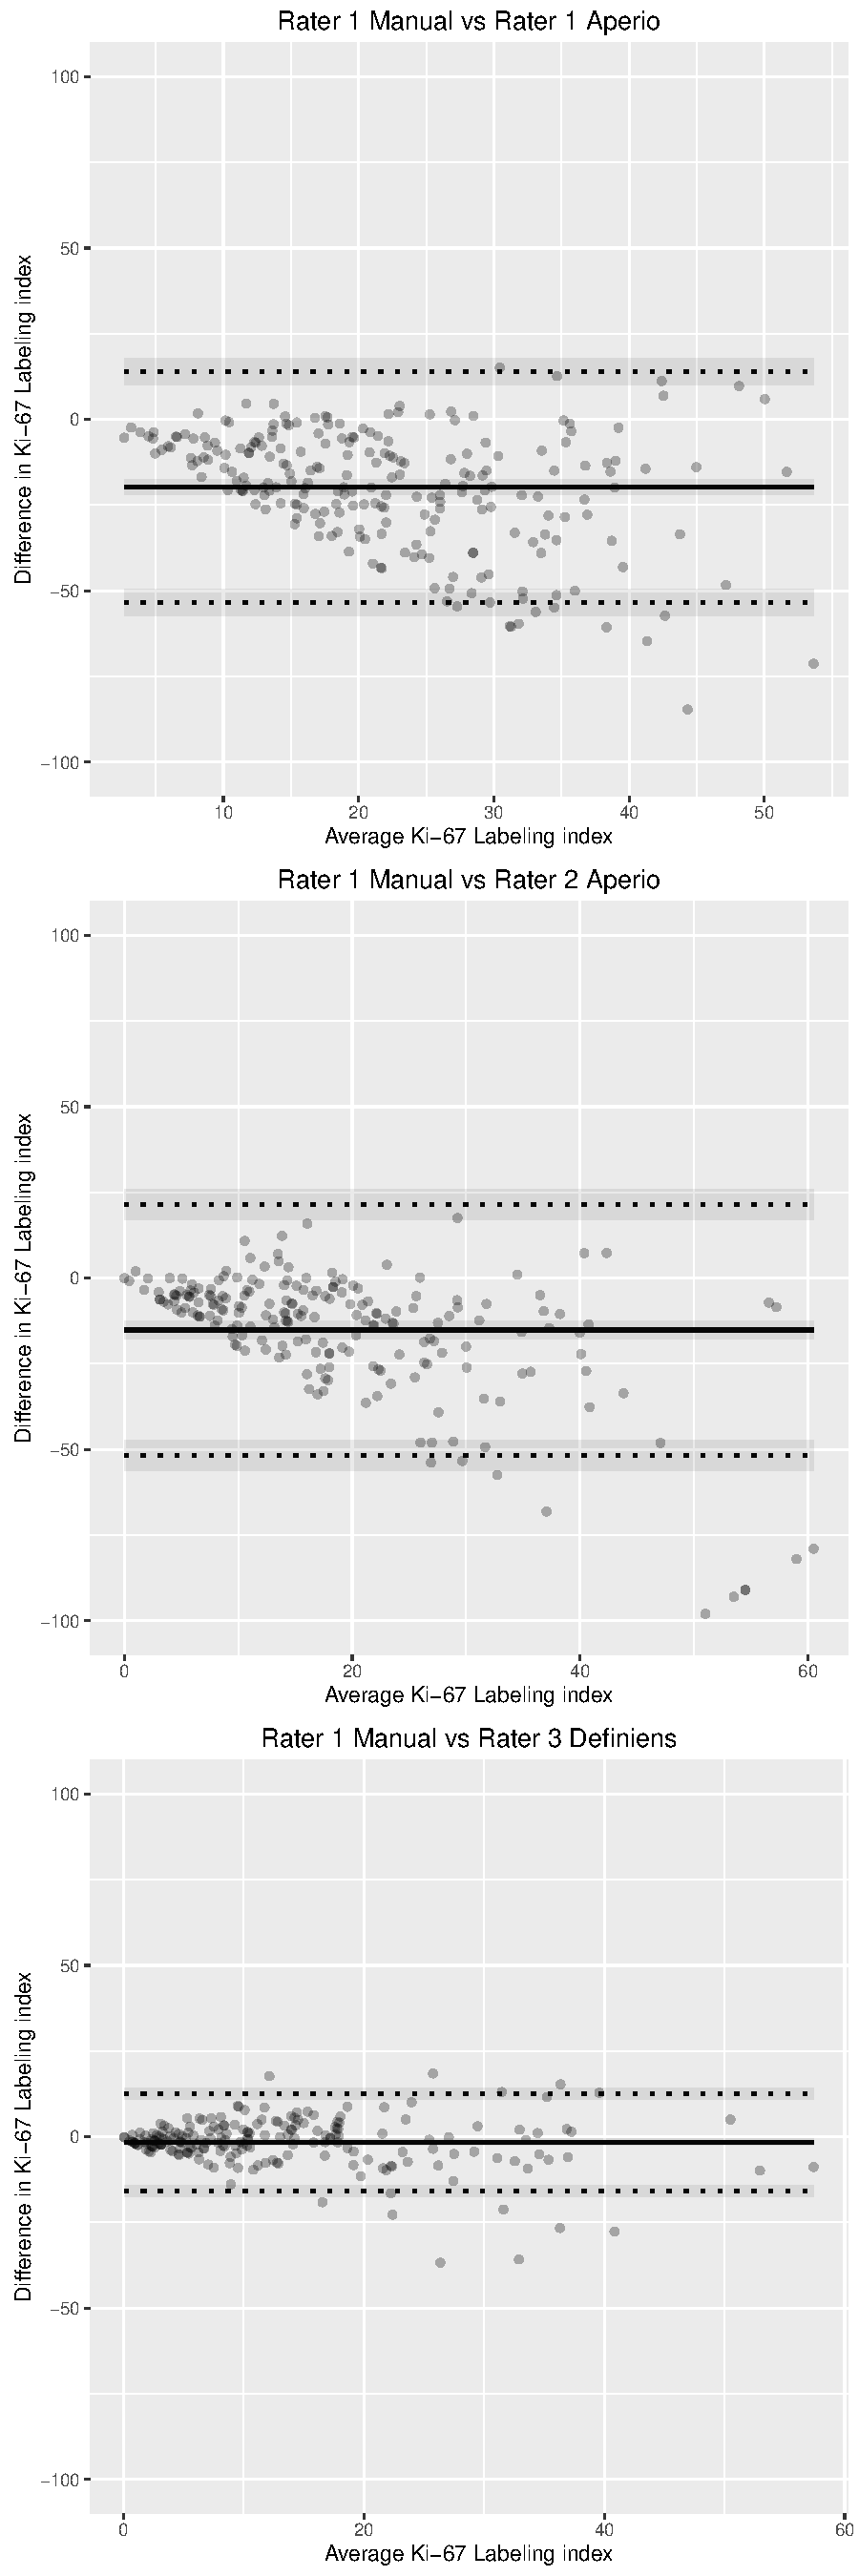
\includegraphics[width = 7cm]{baplot}
\centering
\caption{{\bf Pairwise Bland-Altman Plot}}
\label{baplot}
\end{figure}

\begin{figure}
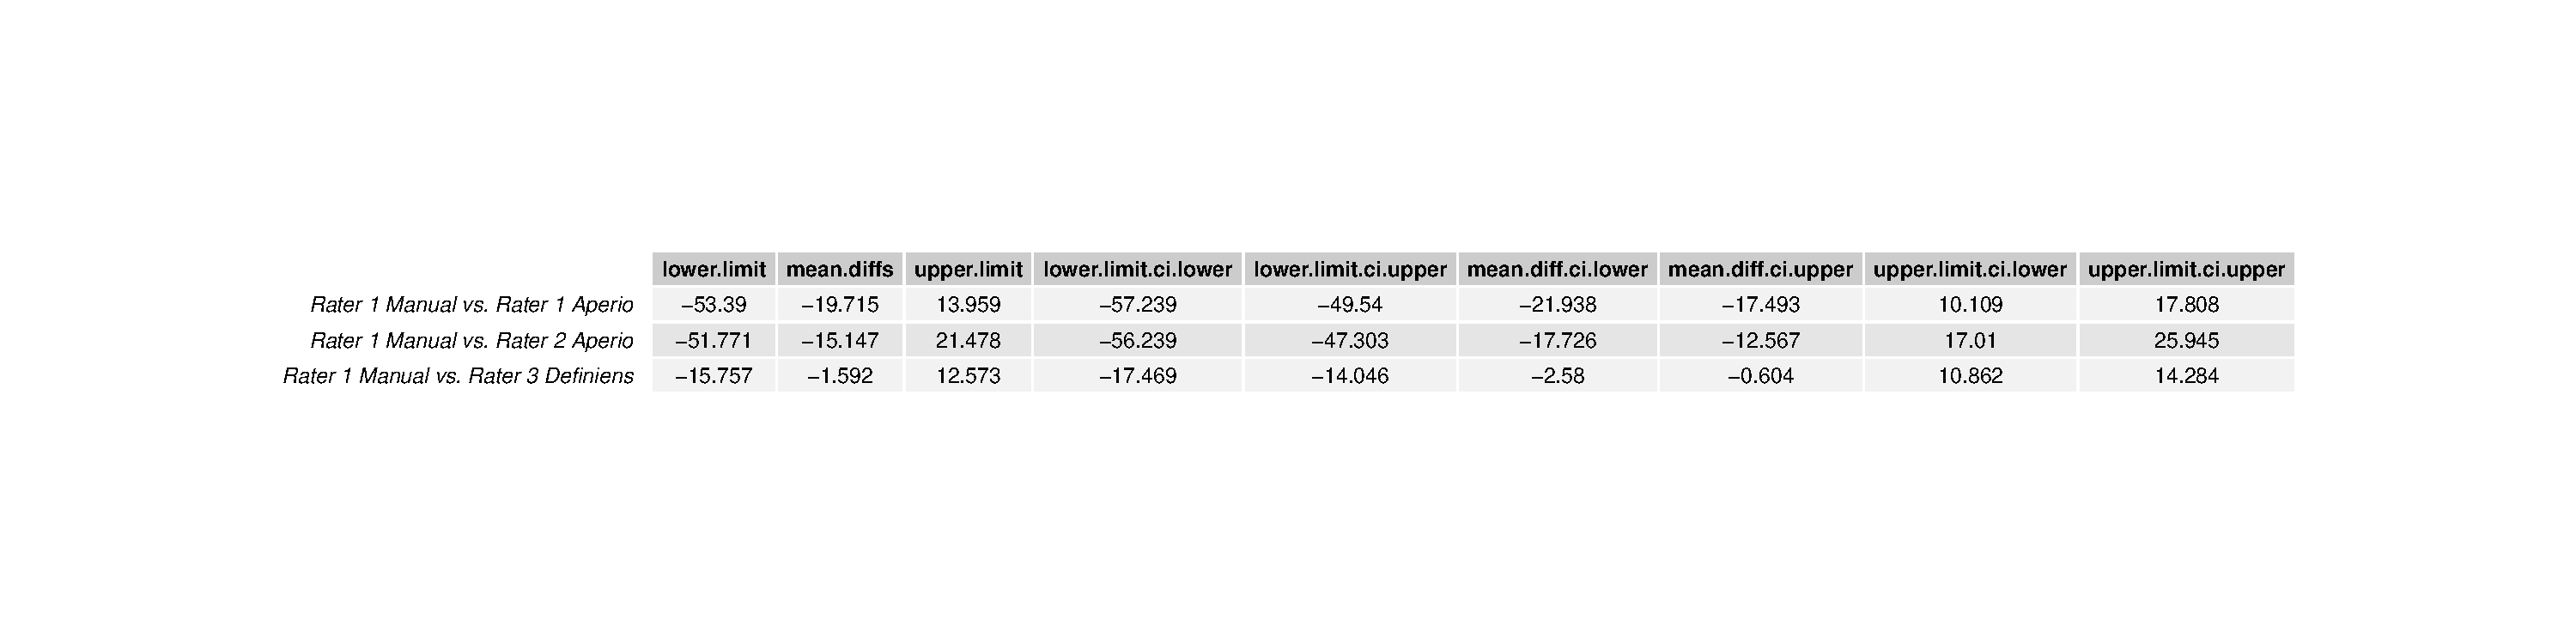
\includegraphics[scale=0.3]{baStat}
\centering
\caption{{\bf Statistics regarding Bland Altman plot}}
\label{baStat}
\end{figure}


\begin{figure}
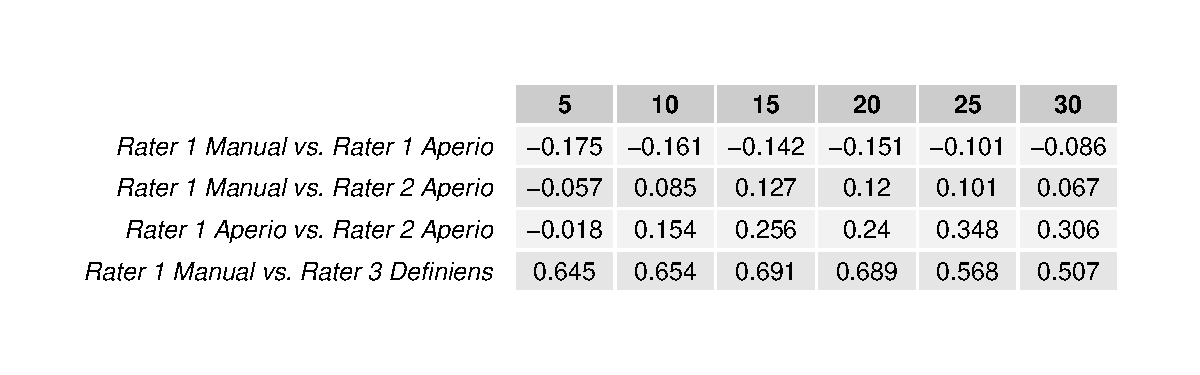
\includegraphics[scale=0.3]{kappaStat}
\centering
\caption{{\bf Kappa statistics }}
\label{kappaStat}
\end{figure}


\end{document}
